\chapter{Introduction}

Music \footnote{Throughout this thesis, "music" refers to the Western tradition, defined by the conventions, practices, and aesthetics that primarily evolved in Europe and North America. This term's usage does not negate the diversity and richness of other musical traditions worldwide. Instead, it specifies this study's concentration on a particular cultural context.}, a cornerstone of human culture, has developed hand in hand with our societies since ancient times. However, its study presents unique challenges due to its subjectivity, fluctuating ground truth, and the vast array of styles and cultural contexts.

Prior research emphasizes the necessity of selecting suitable audio features to distinguish and label unique music segments for music segmentation tasks. The challenge lies in acquiring annotated data for these feature transformations, which can be time-consuming and expensive. In response, scholars have turned to unsupervised deep learning using readily available audio data \cite{deepfeaturesegment, Grill2015MusicAnnotations}. This method has substantially improved the generalization capacity of machine-listening models in downstream applications. Among others, segmentation algorithms have seen significant enhancements and delivered state-of-the-art results \cite{Hernandez-Olivan2021MusicFeatures, Li2023MERT:Training}.

Beyond applications in music structure analysis, the evolution of neural networks has empowered the creation of latent representations \ref{fig:manifold} encapsulating crucial musical traits, technically known as representation ---or feature--- learning. This evolution has simplified the computational process for various task-specific elements, including but not limited to:

\begin{itemize}
\item Creating an audio embedding that excels across numerous applications without the necessity for fine-tuning \cite{Turian2022HEAR:Representations}.
\item Boosting the classification of environmental sounds \cite{CramerLOOKEMBEDDINGS}.
\item Enhancing vocal-centric music tasks through cross-domain audio embeddings \cite{Kim2021LearningLoss}.
\item Integrating task-specific and pre-trained features to optimize audio classification \cite{Hung2022Feature-informedClassification}.
\item Developing a music similarity search engine for video production \cite{epidemic}.
\item Improving Music Emotion Recognition (MER) performance \cite{KohComparisonRecognition}.
\item Evaluating the effectiveness of speaker recognition via pre-trained model embeddings \cite{lightweight}.
\item Embedding songs for artist identification to facilitate similarity comparisons \cite{contentmusicsimtriplet2020}.
\item Addressing cross-modal text-to-music retrieval issues \cite{WonEmotionStories}.
\item Enabling automated music rearrangement \cite{Stoller2018IntuitiveTransitions, Plachouras2023MusicSegmentation}.
\end{itemize}

\begin{figure}[ht]
    \centering
    \scalebox{1.2}{

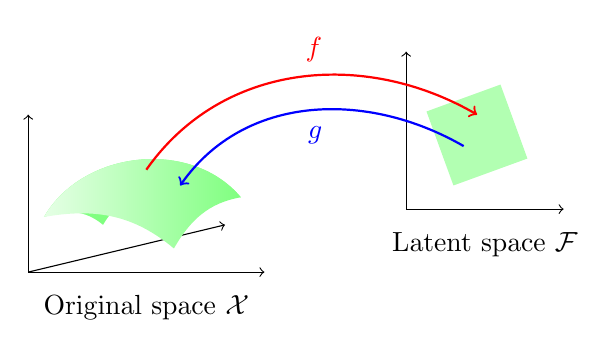
\begin{tikzpicture}
\centering
\draw[->] (0, 0) -- ++(0, 2);
\draw[->] (0, 0) -- ++(2.5, 0.6);
\draw[->] (0, 0) -- ++(3, 0) node[midway, below, yshift=-0.5em]
    {Original space ${\cal X}$};

\draw[fill=green!50, draw=none, shift={(0.2, 0.7)},scale=0.5]
  (0, 0) to[out=20, in=140] (1.5, -0.2) to [out=60, in=160]
  (5, 0.5) to[out=130, in=60]
  cycle;

\shade[thin, left color=green!10, right color=green!50, draw=none,
  shift={(0.2, 0.7)},scale=0.5]
  (0, 0) to[out=10, in=140] (3.3, -0.8) to [out=60, in=190] (5, 0.5)
    to[out=130, in=60] cycle;

  \draw[->] (4.8, 0.8) -- ++(0, 2);
  \draw[->] (4.8, 0.8) -- ++(2, 0) node[midway, below, yshift=-0.5em]
      {Latent space ${\cal F}$};

  \draw[thin, fill=green!30, draw=none, shift={(5.4, 1.1)}, rotate=20]
    (0, 0) -- (1, 0) -- (1, 1) -- (0, 1) -- cycle;

  \draw[thick,->,red]
    (1.5, 1.3) to [out=55, in=150] node[midway, above, xshift=6pt, yshift=2pt]
    {$f$} (5.7, 2);

  \draw[thick,->,blue] (1.5, 1.3) ++(4.03, 0.3) to [out=150, in=55]
    node[midway, below, xshift=2pt, yshift=-2pt] {$g$} ++(-3.6, -0.5);

\end{tikzpicture}}
    
    \caption[Dimensionality reduction and latent space representation \cite{tikz}.]{\small{Dimensionality reduction and latent space representation: Mapping between the original high-dimensional space ${\cal X}$ and the lower-dimensional latent space ${\cal F}$ using functions $f$ and $g$.}}
    \label{fig:manifold}
\end{figure}


Furthermore, deep audio embeddings offer the benefit of transferability, establishing a foundation for multiple tasks. Compared to training a model from scratch, this approach saves computational resources and time \cite{transferMIR2013, CifkaDeepTransfer, Ding2023AudioClassification}.

Unsupervised settings to learn those embeddings confront the persistent challenge of acquiring labeled data, an endeavor often time-consuming and expensive. By capitalizing on the vast volumes of available unlabeled music data, we bypass the need for laborious hand annotation, offering a pathway to potentially more comprehensive generalization.

It is yet to be determined whether a general-purpose audio representation can successfully emulate human hearing \cite{Turian2022HEAR:Representations}, even though some techniques have demonstrated generalizability across many music-understanding tasks \cite{Li2023MERT:Training, Kim2020OneStrategies}. Deep learning's role in music understanding remains relatively nascent, with scarce work on deep music representations, a dearth of large-scale datasets, and a lack of a universal community-driven benchmark \cite{Turian2022HEAR:Representations, Yuan2023MARBLE:Evaluation}.

All in all, given the proven effectiveness of deep audio embeddings in existing research and their potential for transfer learning, they hold considerable promise; therefore, we will leverage deep convolutional neural networks to replace traditional acoustic features with sound-agnostic and content-sensitive embeddings with applications for boundary detection and track segmentation tasks.